\chapter{Implementierung}\label{k_implementierung}
\section{Übersicht über die Klassenhierarchie}
Die in \cref{design_systemueberlick} vorgestellten Komponenten werden durch eine Klassenhierarchie implementiert.
Eine Gesamtübersicht der Klassenhierarchie gibt \cref{uml:class_diagram}.
Im Folgenden werden nun die einzelnen Gruppen genauer betrachtet.
Im Quellcode liegen Klassen derselben Gruppe im gleichen Ordner.

\subsection{Hardware}
Die abstrakte Basisklasse dieser Gruppe ist die \identifier{Component}.
Über sie wird lediglich die entsprechende Pin-Nummer der Komponente zugeordnet.
Von \identifier{Component} erben drei Klassen: \identifier{LED}, \identifier{Sensor} sowie \identifier{Release}:

\begin{itemize}
	\item Die abstrakte Basisklasse \identifier{LED} stellt Methode zum Ein-, Aus- und Umschalten von LEDs bereit.
In den konkreten abgeleiteten Klassen (wie \identifier{GreenLED}) erfolgt dann lediglich noch die Zuordnung zum korrekten PIN.
	\item Bei \identifier{Sensor} handelt es sich ebenfalls um eine abstrakte Basisklasse, die das Abfragen von Sensoren erlaubt.
Ähnlich wie bei den LEDs wird dann in den abgeleiteten Klassen \identifier{PhotoSensor}, \identifier{HallSensor} und \identifier{Trigger} nur noch die PIN-Nummer korrekt gesetzt.
	\item Die konkrete Klasse \identifier{Release} kapselt die konkrete Ansteuerung des Servomotors, und stellt diese über die Methoden \identifier{open()} und \identifier{close()} zur Verfügung.
\end{itemize}

\begin{figure}[hb] \centering
	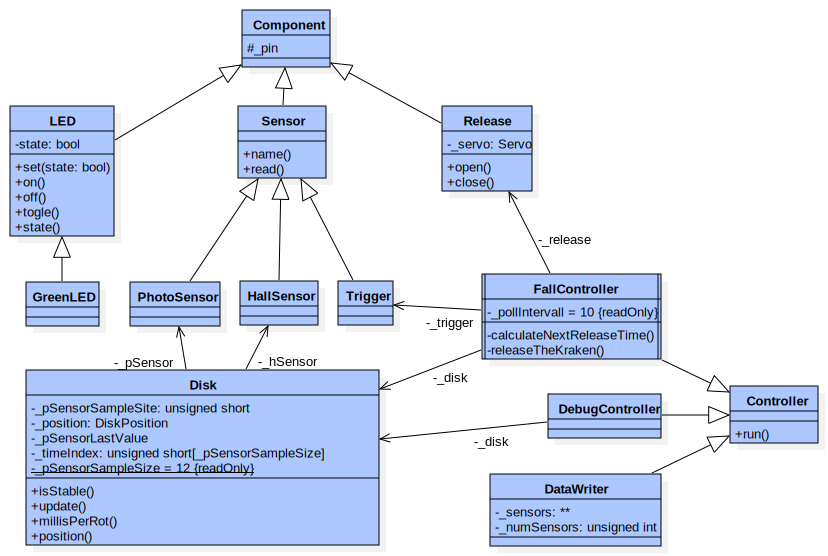
\includegraphics[width=\textwidth]{UML/class_diagram.pdf}
	\caption{Klassendiagramm der Implementierung}
	\label{uml:class_diagram}
\end{figure}

% Kontrollfluss
\begin{figure}[hb] \centering
	\begin{subfigure}[b]{0.4\textwidth}
		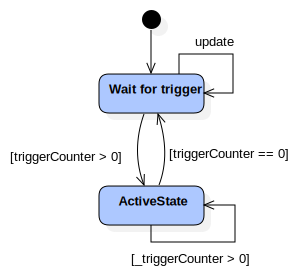
\includegraphics[width=\textwidth]{UML/fallcontroller_simple_loop_statechart.pdf}
		\caption{Einfache Darstellung}
		\label{uml:statechart_simleloop}
	\end{subfigure}\hspace{1cm}
	\begin{subfigure}[b]{0.4\textwidth}
 		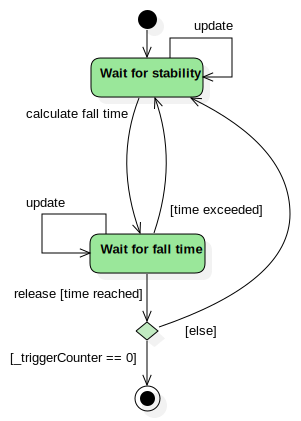
\includegraphics[width=\textwidth]{UML/fallcontroller_active_state_statechart.pdf}
		\caption{Genauere Beschreibung des ActiveStates aus \ref{uml:statechart_simleloop}}
		\label{uml:statechart_activeState}
	\end{subfigure}
	\caption{Beschreibung der Hauptschleife als Zustandsübergangsdiagramm}
	\label{uml:statechart}
\end{figure}

\begin{figure}[hb] \centering
\end{figure}

\begin{figure}[hb] \centering
	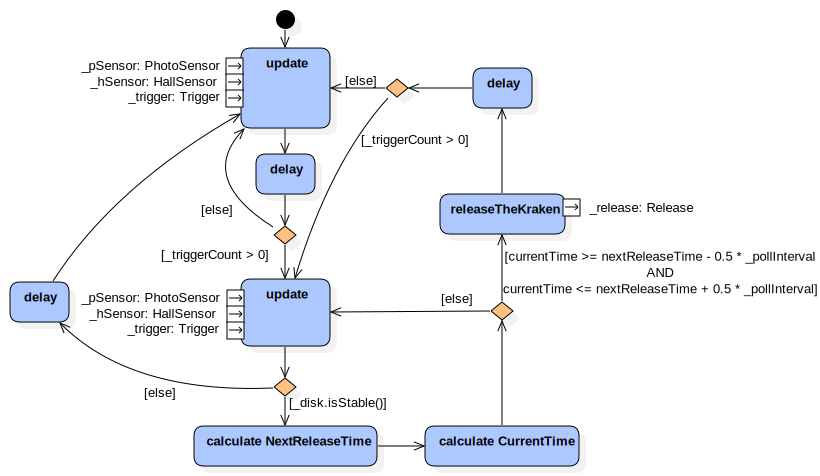
\includegraphics[width=\textwidth]{UML/fallcontroller_loop_activity_diagram.pdf}
	\caption{Genauere Beschreibung der Hauptschleife als Aktivitätsdiagramm}
	\label{uml:activity_diagram}
\end{figure}


% Validierung

%%%%
